\pagebreak
\section{Question 2}
	
	\subsection{Obtaining Obstacle Location from Laser Data}
	
	First we start by taking the data output from question one, which consisted of the robot ${x-y}$ coordinates in the world coordinate system, as well as the velocity and turn rate for that particular timestamp, for each timestamp that occurs in the Velocity observation data, the Compass data and the GPS data. \newline Similar to the way question one works, we combine this data with the Laser observation data by comparing timestamps, using the Prediction Stage equation to estimate the robots {${x-y}$ coordinates at the time that the laser data was generated. Combining the robots ${x-y}$ world coordinates with the relative position of the obstacles obtained from the Laser data. \newline
	For initial tests to attempt to identify obstacles, any range reading from the Laser data that was less than eight (the maximum range of the sensor) was considered an obstacle. It was intended to apply filters to this data once the Occupancy Grid had been generated. Until then, raw data would be used.\newline
	\pagebreak
	The matlab code is shown below:
	\lstinputlisting{./code/q2/q2_obtain_obstacles.m}
		
%	\begin{figure}[position = here]
%		\begin{centering}
%			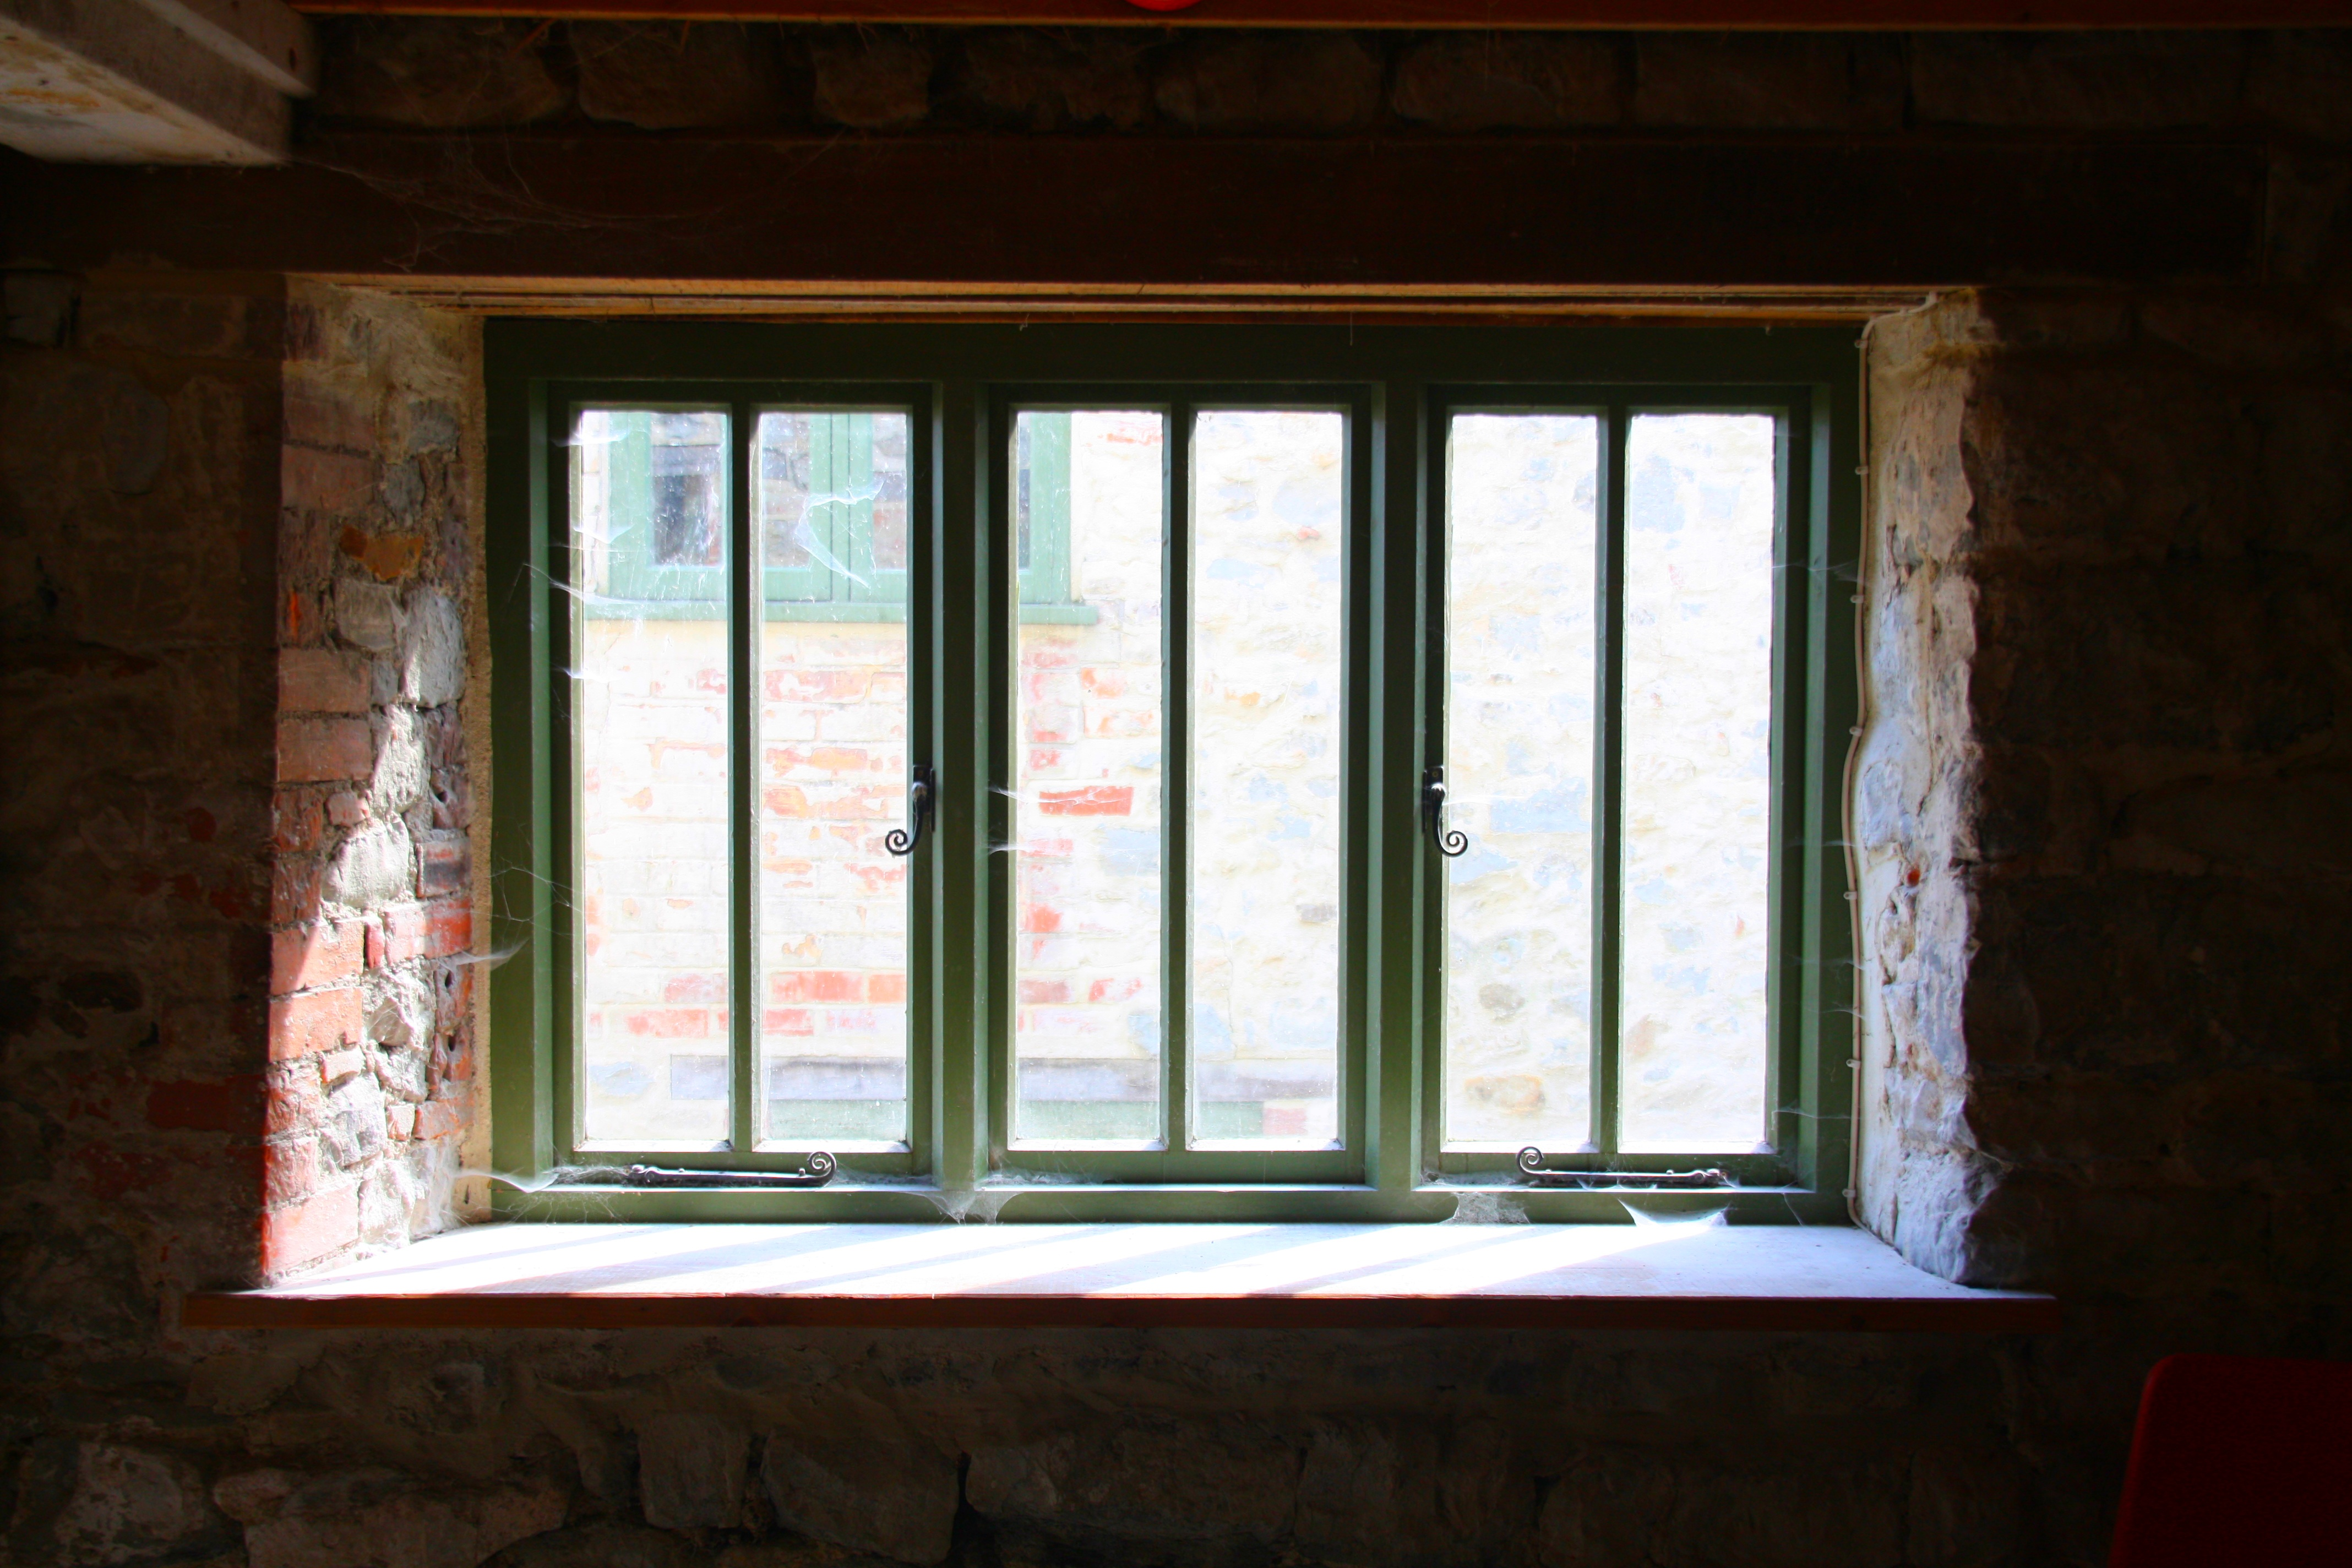
\includegraphics[scale=0.05]{wallWindow}\\
%			\caption[\textit{RPYAxes}]{}
%		\end{centering}
%	\end{figure}
%	\newline
	
	
	\subsection{Generate Occupancy Grid}
	To generate the Occupance Grid, we took the Data set of the X-Y coordinates of all 'Obstacles' detected, and determined the difference between the minimum and maximum ${x}$ and ${y}$ values deteced. Given a user defined size for the occupancy grid, we could then determine the ${x-y}$ range that corresponded to a grid location. Then for every Obstacle ${x-y}$ coordinate we could determine the grid location it corresponded to, incrementing the grid value to increase the weighting, which would indicate the likelihood of an obstacle being in that region. Some experimenting with the grid size using the data for the Robot path generated in question one indicated that a grid size of ${200x200}$ would be best, as this resulted in a grid map that, while not extremely sharp, was also not extremely blurred. Ideally, the grid would be vague enough to generalise a position for the obstacles, but not so clear that it simply resulted in a plot of every possible obstacle coordinates. See the figures below:\newline 
	
		\begin{figure}[position = here]
			\begin{centering}
				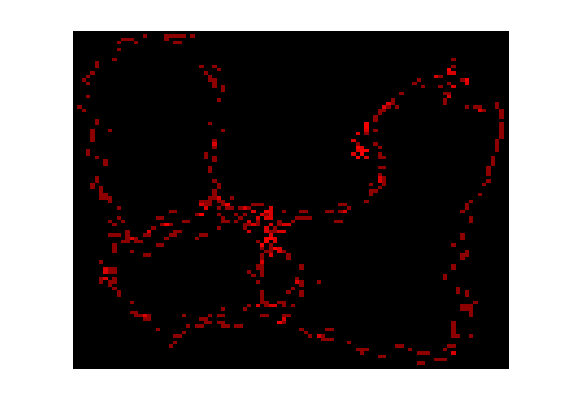
\includegraphics[scale=1]{./images/q2/heatmap_path_100.png}\\
				\caption{Grid size = ${100 \times 100}$}
			\end{centering}
		\end{figure}
		\newline
		
		\begin{figure}[position = here]
			\begin{centering}
				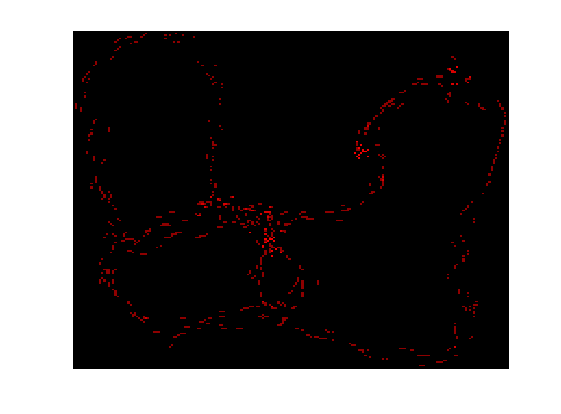
\includegraphics[scale=1]{./images/q2/heatmap_path_200.png}\\
				\caption{Grid size = ${200 \times 200}$}
			\end{centering}
		\end{figure}
		\newline
		
		\begin{figure}[position = here]
			\begin{centering}
				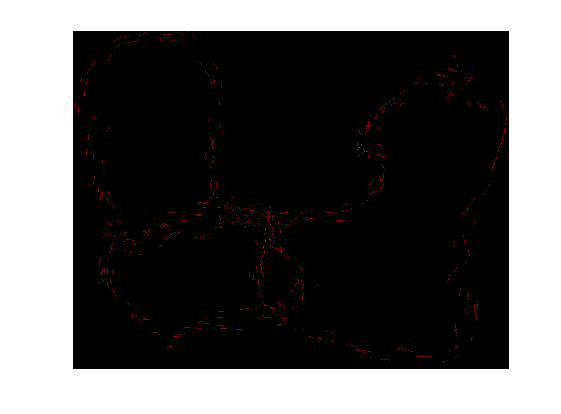
\includegraphics[scale=1]{./images/q2/heatmap_path_500.png}\\
				\caption{Grid size = ${500 \times 500}$}
			\end{centering}
		\end{figure}
		\newline
		\pagebreak
		The matlab code for the occupancy grid is shown below:
		\lstinputlisting{./code/q2/occupancy_grid.m}
	
		\pagebreak
	\subsection{Results}
		The main problem with generating the obstacle data is that the program used took far to long to run. In order to find the obstacles detected for each timestamp, the program took nearly forty minutes to run. The text file containing the laser observation data was nearly eight megabytes in size, so a long run time was expected, however the actual time taken was excessive. In order to get results in a appropriate time, the code was modified to iterate through the timestamps in jumps of twenty, resulting in a run time of a few minutes. Although this would reduce the accuracy of the robot location slightly, the tradeoff was considered acceptable to get an output in a decent timeframe.\newline
		The second problem came when the obstacle location data was compiled into a heatmap. See the images below:\newline
		
				\begin{figure}[position = here]
					\begin{centering}
						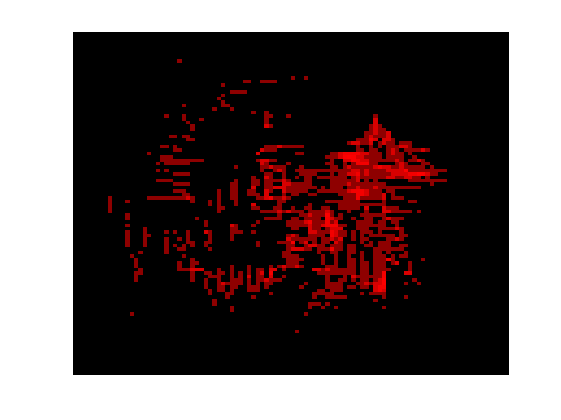
\includegraphics[scale=1]{./images/q2/heatmap_obstacles_200.png}\\
						\caption{Grid size = ${200 \times 200}$}
					\end{centering}
				\end{figure}
				\newline
				
				\begin{figure}[position = here]
					\begin{centering}
						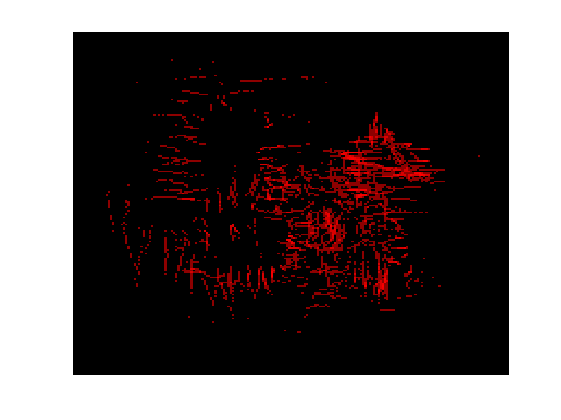
\includegraphics[scale=1]{./images/q2/heatmap_obstacles_500.png}\\
						\caption{Grid size = ${500 \times 500}$}
					\end{centering}
				\end{figure}
				\newline
				\pagebreak
		
		As can be seen, the obstacles are not accurately generated. It appears as if the obstacles/walls detected are in fact rotating. This suggests a flaw in the conversion between the robots coordinate system and the world coordinate system. The code lines that governed this are shown below:
		\lstinputlisting{./code/q2/convert_to_world.txt}		
		\pagebreak
		\newline
		Given the issues with the original code in regards to runtime, as well as the issues converting to the correct coordinate system, we decided to re-write the code to generate obstacle data. To do this, we utilised the laserShowAcfr.m file given for Assignment 2 and adapt it slightly to fit in our timestamp matching system. The resulting code is shown below:
		\lstinputlisting{./code/q2/q2_obtain_obstacles_attempt2.m}
		\pagebreak
		\newline
		This code was able to run for every timestamp in less than a minute. It was deduced that the reason for this is that, for the original code, we were reading the entire range reading from the laserObs.txt file into a matrix at the beginning of the program. This resulted in a matrix of size ${2836 \time 362}$, filled with doubles. This took up a large amount of memory, and caused accessing it to take huge amounts of time. The laserShowAcfr.m code from Assignment 2 instead only read a single line from the laserObs.txt at the time at which operations occurred on it, severly reducing the memory used, allowing the program to execute much faster.\newline
		Despite this breakthrough, we still had issues. The resulting occupancy grid can be found below:
		\begin{figure}[position = here]
			\begin{centering}
				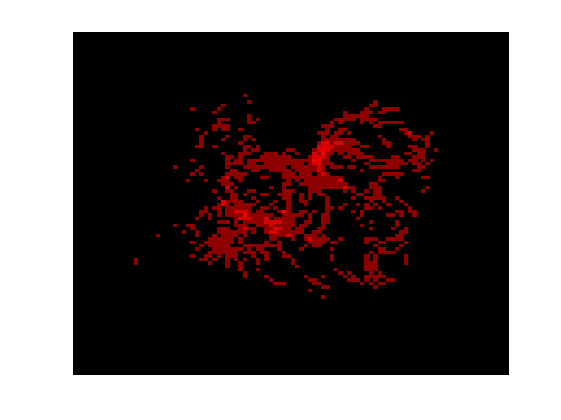
\includegraphics[scale=1]{./images/q2/heatmap_attempt2.png}\\
				\caption{Grid size = ${200 \times 200}$}
			\end{centering}
		\end{figure}
		\newline
		
		Obviously this is still not correct. Going through frame-by-frame, we can see the reason why:
		
		\pagebreak
		\begin{figure}[position = here]
			\begin{centering}
				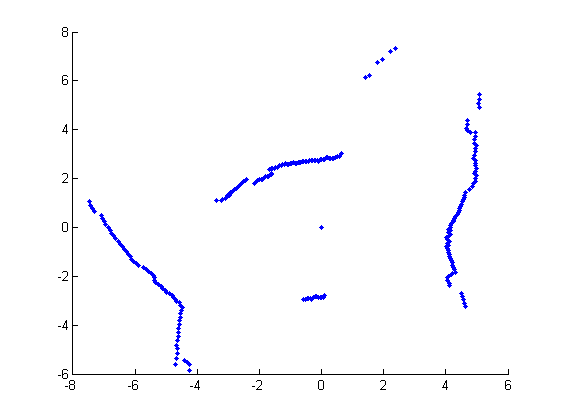
\includegraphics[scale=1]{./images/q2/wall_1_attempt2.png}\\
				\caption[\textit{RPYAxes}]{}
			\end{centering}
		\end{figure}
		\newline
		\pagebreak
		
		\begin{figure}[position = here]
			\begin{centering}
				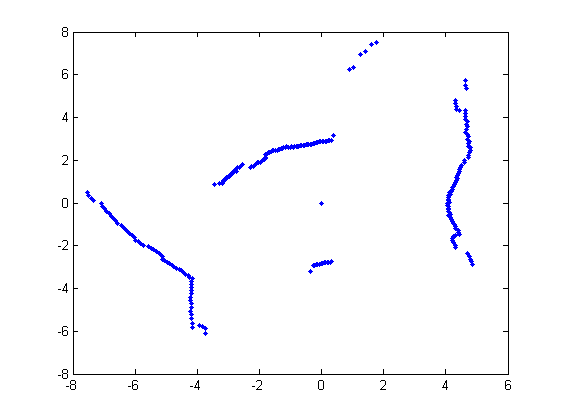
\includegraphics[scale=1]{./images/q2/wall_2_attempt2.png}\\
				\caption[\textit{RPYAxes}]{}
			\end{centering}
		\end{figure}
		\newline
		\pagebreak
		
		\begin{figure}[position = here]
			\begin{centering}
				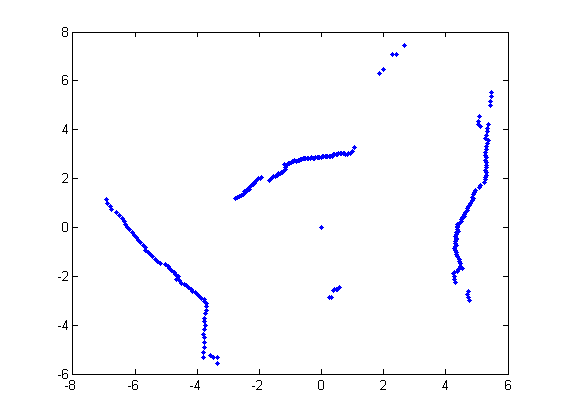
\includegraphics[scale=1]{./images/q2/wall_3_attempt2.png}\\
				\caption[\textit{RPYAxes}]{}
			\end{centering}
		\end{figure}
		\newline
		\pagebreak

		\begin{figure}[position = here]
			\begin{centering}
				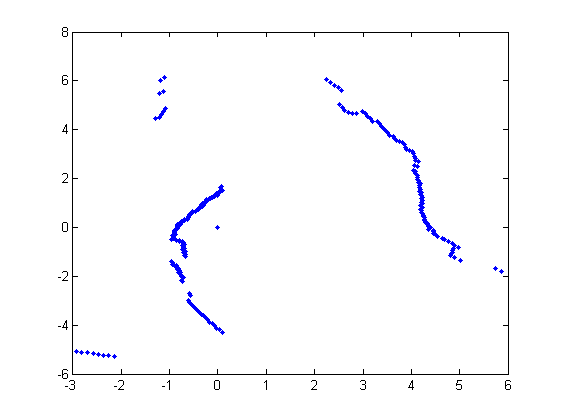
\includegraphics[scale=1]{./images/q2/wall_5_attempt2.png}\\
				\caption[\textit{RPYAxes}]{}
			\end{centering}
		\end{figure}
		\newline
		\pagebreak
				
		\begin{figure}[position = here]
			\begin{centering}
				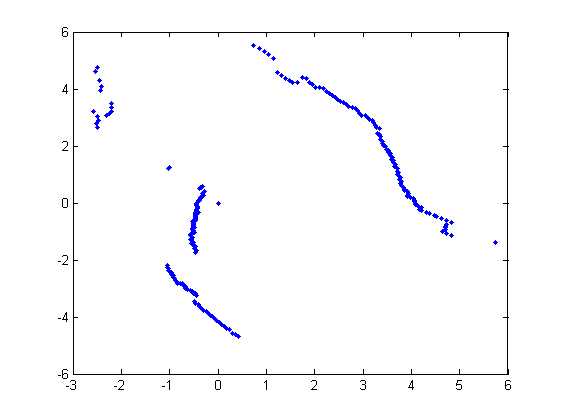
\includegraphics[scale=1]{./images/q2/wall_6_attempt2.png}\\
				\caption[\textit{RPYAxes}]{}
			\end{centering}
		\end{figure}
		\newline
		
		\pagebreak

		
						
		The obstacles detected can be seen to be rotating. Obviously, once again, there is an issue with converting from the robots coordinate system to real-world coordinates.\newline The lines in the new code governing this are shown below:
		
		\lstinputlisting{./code/q2/convert_to_world_2.txt}
		\newline
		
		
		Upon closer analysis, it was determined that the flaw is that we are attempting to go straight from range and bearing to the real world coordinate system. Because of this, we are missing out on several crucial steps. This particularly effects the rotation. The method that should have been used is shown below:
		\lstinputlisting{./code/q2/convert_to_world_actual.txt}
		\newline
		The crucial part that was missing from our code is at lines 8 and 9 in the above code snippet. When rotating the x and y values from the robots frame of reference, we are not taking into account the ${\sin}$ offset for our ${x}$ values, and the ${\cos}$ offset for our ${y}$ values. This results in the final ${x-y}$ coordinates still being partially in the robots reference frame, giving rise to the observed rotation.
		
		
		
		
		
		
		
		
		
		